\documentclass[12pt]{article}
\usepackage{geometry}
\geometry{a4paper, portrait, margin=1in}

% --- Math Packages ---
\usepackage{amsmath}
\usepackage{amssymb}
\usepackage{amsfonts}
\usepackage{amsthm}

% --- Graphics & Diagrams ---
\usepackage{graphicx}
\usepackage{tikz}
\usetikzlibrary{shapes, arrows, positioning}

% --- Formatting ---
\usepackage{parskip}
\usepackage[hidelinks]{hyperref}
\usepackage{natbib}
\usepackage{enumitem}
\pagestyle{plain}

% --- Word count (requires compiling with --shell-escape) ---
\newcommand{\wordcount}{%
  \immediate\write18{texcount -sum -1 \jobname.tex 2>/dev/null | python3 -c "import sys; n=sys.stdin.read().strip(); print(f'{int(n):,}') if n.isdigit() else print('?')" > \jobname.wc}%
  \input{\jobname.wc}%
}

% --- Theorem environments ---
\newtheorem{proposition}{Proposition}
\newtheorem{corollary}{Corollary}
\newtheorem{result}{Result}

\title{TT Week 1 Model}
\author{Mohammad-Shah Karim}
\date{April 2026}

\begin{document}

\maketitle

\begin{center}
  \small Word count: \wordcount
\end{center}

\tableofcontents

\newpage

\section{Introduction}

This document outlines a game-theoretical model for pharmaceutical innovation and pricing to explain the empirical puzzle observed in the patent market following the expansion of Medicaid under the Affordable Care Act. The model captures the stochastic nature of R\&D, the specific procurement mechanism (PDL bidding) used by state agencies, and how current procurement outcomes dictate future innovation incentives.

The model is set up for a representative therapeutic class $c \in \mathcal{C}$, where $\mathcal{C}$ denotes the set of ATC Level 1 classes. Each class is characterised by a class-specific Medicaid market size $M_c$, a class-specific rebate function $\tau_c(M_c)$, and a degree of therapeutic substitutability $n_c$. The innovation and clinical approval stages (Stages 1-2) are common across classes; the pricing subgame (Stage 3) and all downstream equilibrium analysis are class-indexed. This structure is motivated by the triple-difference results (RQ3), which reveal that the expansion's effect on innovation varies sharply across therapeutic areas.

Figure \ref{fig:game_structure} summarises the sequence of play, mapping the innovation decision in Period 1 to the pricing outcomes, which subsequently define the firm's state for future investment decisions in Period 2.

\begin{figure}[h]
    \centering
    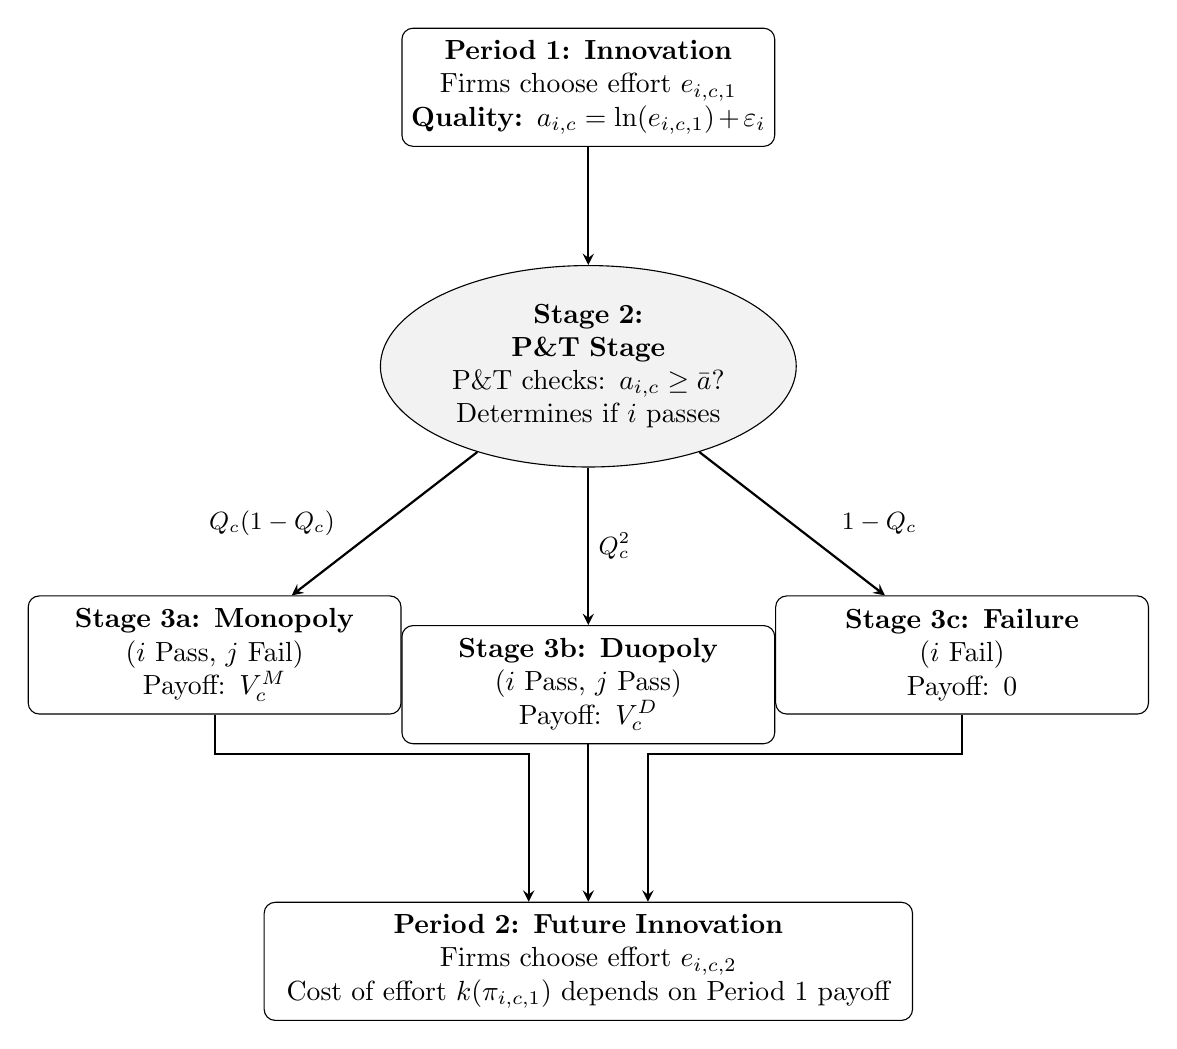
\begin{tikzpicture}[
        node distance=1.5cm and 1cm,
        auto,
        block/.style={rectangle, draw, fill=white, text width=4.5cm, align=center, rounded corners, minimum height=1.5cm},
        wideblock/.style={rectangle, draw, fill=white, text width=8cm, align=center, rounded corners, minimum height=1.5cm},
        cloud/.style={ellipse, draw, fill=gray!10, text width=3.5cm, align=center, minimum height=1.2cm},
        arrow/.style={thick,->,>=stealth}
    ]

    % Stage 1: Innovation
    \node [block] (stage1) {\textbf{Period 1: Innovation}\\ Firms choose effort $e_{i,c,1}$\\ \textbf{Quality:} $a_{i,c} = \ln(e_{i,c,1}) + \varepsilon_i$};

    % Stage 2: P&T Stage
    \node [cloud, below=of stage1] (pt) {\textbf{Stage 2: P\&T Stage}\\ P\&T checks: $a_{i,c} \ge \bar{a}$?\\ Determines if $i$ passes};
    
    % Monopoly
    \node [block, below left=2cm and 0.5cm of pt] (mono) {\textbf{Stage 3a: Monopoly}\\ ($i$ Pass, $j$ Fail)\\ Payoff: $V_c^M$};
    
    % Duopoly
    \node [block, below=2cm of pt] (duo) {\textbf{Stage 3b: Duopoly}\\ ($i$ Pass, $j$ Pass)\\ Payoff: $V_c^D$};
    
    % Failure
    \node [block, below right=2cm and 0.5cm of pt] (fail) {\textbf{Stage 3c: Failure}\\ ($i$ Fail)\\ Payoff: $0$};

    % Period 2
    \node [wideblock, below=2cm of duo] (period2) {\textbf{Period 2: Future Innovation}\\ Firms choose effort $e_{i,c,2}$ \\ Cost of effort $k(\pi_{i,c,1})$ depends on Period 1 payoff};

    % Connecting Lines
    \draw [arrow] (stage1) -- (pt);
    \draw [arrow] (pt) -- node[left, xshift=-0.5cm, font=\small] {$Q_c(1-Q_c)$} (mono);
    \draw [arrow] (pt) -- node[font=\small] {$Q_c^2$} (duo);
    \draw [arrow] (pt) -- node[right, xshift=0.5cm, font=\small] {$1-Q_c$} (fail);
    
    \draw [arrow] (mono.south) -- ++(0,-0.5) -| (period2.135);
    \draw [arrow] (duo.south) -- (period2.north);
    \draw [arrow] (fail.south) -- ++(0,-0.5) -| (period2.45);

    \end{tikzpicture}
    \caption{The Sequence of Play in Class $c$: Innovation, P\&T Approval, Pricing, and Future Investment}
    \label{fig:game_structure}
\end{figure}

\newpage

\section{Stage 1: The Innovation Decision (Effort)}

First, firms make investment decisions for a drug they wish to market in therapeutic class $c$. Innovation is modelled to require effort --- this is costly but improves the probability of clinical success.

\subsection{The Production Technology}
The realised clinical quality $a_{i,c}$ is a function of the effort exerted by the firm and a stochastic component $\varepsilon_i$:
\begin{equation}
    a_{i,c} = \ln(e_{i,c}) + \varepsilon_i, \qquad \varepsilon_i \sim N(0, \sigma^2)
\end{equation}
where $\varepsilon_i$ represents the inherent uncertainty of the R\&D process.

\subsection{The Cost of Effort}
Firms $i$ and $j$ simultaneously choose R\&D effort levels $e_{i,c} \geq 0$ within class $c$. Effort is assumed to be costly and convex:
\begin{equation}
    C(e_{i,c}) = \frac{1}{2} k \, e_{i,c}^2
\end{equation}

\newpage

\section{Stage 2: The P\&T Stage}
Once effort is exerted it is now a sunk cost, nature determines the clinical outcome of each firm's drug $a_{i,c}$, i.e.\ whether the drug passes the P\&T stage.

\subsection{The Approval Condition}
A drug is clinically approved (passes the P\&T stage) if its quality $a_{i,c}$ exceeds a regulatory threshold $\bar{a}$:
\begin{equation}
    \text{P\&T Stage}_{i,c} = 
    \begin{cases} 
        \text{Approved} & \text{if } a_{i,c} \geq \bar{a} \\
        \text{Not Approved} & \text{if } a_{i,c} < \bar{a}
    \end{cases}
\end{equation}

\subsection{The Probability of Success \texorpdfstring{($Q_c$)}{(Qc)}}
The probability of passing in class $c$, denoted $Q_c(e_{i,c})$, is endogenous to effort:
\begin{align}
    Q_c(e_{i,c}) &= \Pr(\ln e_{i,c} + \varepsilon_i \geq \bar{a}) \\
           &= \Pr(\varepsilon_i \geq \bar{a} - \ln e_{i,c}) \\
           &= 1 - \Pr(\varepsilon_i < \bar{a} - \ln e_{i,c}) \\
           &= 1 - \Phi\left(\frac{\bar{a} - \ln e_{i,c}}{\sigma}\right)
\end{align}
where $\Phi(\cdot)$ is the standard normal CDF. \vspace{1em}

This defines the transition probabilities into Stage 3.

\newpage

\section{Stage 3: The Pricing Subgame}
Firms that pass Stage 2 compete for market access within therapeutic class $c$. Each class $c$ is characterised by three primitives:

\begin{enumerate}[label=(\roman*)]
    \item A class-specific Medicaid market size $M_c$, which increases following the ACA expansion by $\Delta M_c \geq 0$. Classes with a higher pre-expansion Medicaid share experience larger shocks.
    
    \item A class-specific rebate function $\tau_c(M_c)$ with $\tau_c' > 0$, governing how aggressively the state can extract supplemental rebates in class $c$. This is a reduced-form representation of supplemental rebate negotiations under U.S. Medicaid's multi-state pooling institutions (see the Institutional and Empirical Justification subsection), not a general law: $\tau_c(M_c)$ captures the per-unit rebate the state extracts in expectation, denominated in dollars per Medicaid prescription.
    
    \item A measure of therapeutic substitutability $n_c \geq 1$, defined as the number of clinically interchangeable molecules available to the PDL committee within class $c$.
\end{enumerate}

The model imposes no specific functional form on $\tau_c$; the only structural requirement is $\tau_c' > 0$. To introduce cross-class heterogeneity, we assume that the steepness of the rebate schedule is linked to the degree of therapeutic substitutability:
\begin{equation} \label{eq:tau_steepness}
    \tau_c'(M_c) \text{ is increasing in } n_c
\end{equation}

That is, classes with more therapeutic substitutes face steeper rebate schedules. When a PDL committee has many clinically interchangeable molecules to choose from, it can credibly threaten to exclude any given manufacturer unless a deeper rebate is offered. Classes with more substitutes (higher $n_c$) therefore have steeper rebate schedules because the state's outside option in procurement negotiations is stronger. Specific functional forms for $\tau_c$ are adopted only for the comparative statics simulations (Section \ref{sec:comp_statics}).

The game resolves into one of three mutually exclusive states.

\subsection{Stage 3a: The Monopoly State}

\textbf{Condition:} Firm $i$ passes while firm $j$ fails:
\begin{align*}
    a_{i,c} \geq \bar{a} > a_{j,c}
\end{align*}

\textbf{Mechanism:} Firm $i$ is the sole player in class $c$ and negotiates directly with the state.

\paragraph{Setup} 
The firm faces a class-specific market demand $M_c$ which is perfectly inelastic with respect to price. Because Medicaid enrollees are fully insured with negligible out-of-pocket cost-sharing, we assume demand is completely inelastic up to the population limit $M_c$, a standard assumption in the literature modelling public insurance procurement. However, the state imposes a maximum allowable price $\bar{p}$ and the firm also pays the class-specific rebate $\tau_c(M_c)$.

\paragraph{Optimisation Problem}
The firm chooses price $p$ to maximise profit:
\begin{equation}
    \max_{p} \pi_{i,c} = M_c(p - c_i - \tau_c(M_c)) \quad \text{s.t.} \quad p \le \bar{p}
\end{equation}
Since demand is inelastic, the profit function is strictly increasing in $p$.

\paragraph{Equilibrium Result}
The firm sets the price at the binding cap: $p^* = \bar{p}$, and the resulting profit is:
\begin{equation} \label{eq:mono_profit}
    \pi_{i,c}^{Mono}(c_i) = M_c(\bar{p} - c_i - \tau_c(M_c))
\end{equation}
Denote the expected value of this state across marginal costs as: 
\begin{equation}
V_c^M = \mathbb{E}_c[\pi_{i,c}^{Mono}]
\end{equation}

\subsection{Stage 3b: The Duopoly State (Auction)}
\textbf{Condition:} Both firms pass the P\&T stage in class $c$:
\begin{align*}
    a_{i,c} \geq \bar{a}, \qquad a_{j,c} \geq \bar{a}
\end{align*}

\textbf{Mechanism:} Firms compete in a first-price sealed-bid procurement auction.

\paragraph{Setup}
Each firm independently draws a marginal cost $c_i, c_j$ from a common distribution $F(c)$ with support $[\underline{c}, \bar{c}]$. Each firm submits a sealed bid (net price) $b_i$. The lowest bidder wins PDL status in class $c$ and obtains the full market volume $M_c$ minus the class-specific statutory wedge $\tau_c(M_c)$.
\[
\pi_{i,c} =
\begin{cases}
M_c\big(b_i - c_i - \tau_c(M_c)\big) & \text{if } b_i \leq b_j, \\
0 & \text{if } b_i > b_j.
\end{cases}
\]

\paragraph{Equilibrium Derivation}
Assume that there exists a strictly increasing and differentiable symmetric Bayesian-Nash Equilibrium bidding strategy $b_c(c)$.

\subparagraph{Step 1: The Probability of Winning}
Suppose firm $i$ has cost $c$ but considers submitting a bid $\tilde{b}$ corresponding to the optimal bid of type $t$ (i.e., $\tilde{b} = b_c(t)$). Firm $i$ wins if its bid is lower than the rival's bid $b_c(c_j)$:
\begin{equation}
    b_c(t) < b_c(c_j) \iff t < c_j
\end{equation}
The probability of winning is therefore:
\begin{equation}
    \Pr(\text{win}) = \Pr(c_j > t) = 1 - F(t)
\end{equation}

\subparagraph{Step 2: The Optimisation Problem}
The firm chooses the target type $t$ to maximise expected profit:
\begin{equation}
    \max_{t} \mathbb{E}[\pi_{i,c}(t, c)] = M_c(b_c(t) - c - \tau_c(M_c))[1 - F(t)]
\end{equation}
Let $U_c(c)$ be the value function (maximum expected profit) for a firm with true cost $c$ in class $c$:
\begin{equation}
    U_c(c) = \max_{t} M_c(b_c(t) - c - \tau_c(M_c))[1 - F(t)]
\end{equation}

\subparagraph{Step 3: Applying the Envelope Theorem}
Differentiation of the value function $U_c(c)$ with respect to cost $c$ yields the partial derivative of the objective function evaluated at the optimal choice $t=c$ (truth-telling):
\begin{equation}
    U_c'(c) = \left. \frac{\partial \mathbb{E}[\pi_{i,c}(t, c)]}{\partial c} \right|_{t=c} = -M_c[1 - F(c)]
\end{equation}

\subparagraph{Step 4: Solving for Expected Profit}
Integrating $U_c'(c)$ from $c$ to $\bar{c}$, and noting that profit at the highest cost type $U_c(\bar{c}) = 0$:
\begin{equation} \label{eq:value_integral}
    U_c(c) = M_c \int_{c}^{\bar{c}} (1 - F(u)) \, du
\end{equation}

\subparagraph{Step 5: Recovering the Bidding Function}
Equating the integral expression (\ref{eq:value_integral}) with the definition of profit at the optimum yields the symmetric equilibrium bidding strategy:
\begin{equation} \label{eq:bid_function}
    b_c(c) = c + \tau_c(M_c) + \frac{\int_{c}^{\bar{c}} (1 - F(u)) \, du}{1 - F(c)}
\end{equation}

\paragraph{Equilibrium Result (Expected Payoff)}
Substituting the optimal bid, the ex-ante expected profit for entering Stage 3b in class $c$ is:
\begin{equation} \label{eq:duo_profit}
    \Pi_c^{Duo}(c) = M_c \int_{c}^{\bar{c}} (1 - F(u)) \, du
\end{equation}

Denote the expected value of this state across marginal costs as: 
\begin{equation}
V_c^D = \mathbb{E}_c[\Pi_c^{Duo}]    
\end{equation}

Note that $V_c^D$ scales linearly with $M_c$ and is unaffected by the rebate wedge $\tau_c(M_c)$, since auction competition drives the effective price to cost. This asymmetry between $V_c^M$ and $V_c^D$ in their dependence on $\tau_c$ is central to the incentive trap mechanism.

\subsection{Stage 3c: The Failure State}
\textbf{Condition:} Firm $i$ fails in class $c$:
\begin{align*}
    a_{i,c} < \bar{a}
\end{align*}

The firm fails to meet the clinical threshold required for PDL consideration. It cannot submit a bid.

\paragraph{Equilibrium Result}
The firm does not enter the market and earns zero revenue.
\begin{equation}
    \pi_{i,c}^{Fail} = 0
\end{equation}

\newpage

\section{Equilibrium Analysis}
Solve for the equilibrium within each therapeutic class $c$ by examining the optimal contemporaneous effort, and subsequently modelling how current procurement outcomes shape future innovation.

\subsection{The Maximisation Problem}
Within class $c$, the firm chooses effort $e_{i,c}$ to maximise total expected profit, where $\Psi_{i,c}$ is the probability-weighted sum of payoffs in each state minus the cost of effort:
\begin{equation}
    \max_{e_{i,c}} \Psi_{i,c} = \underbrace{Q_c(e_{i,c})[1-Q_c(e_{j,c})] V_c^M}_{\text{Stage 3a Incentive}} + \underbrace{Q_c(e_{i,c})Q_c(e_{j,c}) V_c^D}_{\text{Stage 3b Incentive}} - \frac{1}{2} k \, e_{i,c}^2
\end{equation}
where $V_c^M$ and $V_c^D$ are the class-specific expected values derived in the monopoly and duopoly cases, respectively.

\subsection{Optimal Effort \texorpdfstring{$(e_c^*)$}{(ec*)}}
The First Order Condition (FOC) with respect to effort $e_{i,c}$ is derived by differentiating $\Psi_{i,c}$:
\begin{equation}
    \frac{\partial \Psi_{i,c}}{\partial e_{i,c}} = Q_c'(e_{i,c})(1-Q_c(e_{j,c})) V_c^M + Q_c'(e_{i,c})Q_c(e_{j,c}) V_c^D - k \, e_{i,c} = 0
\end{equation}
This yields the following expression, where the marginal benefit of effort is equal to the associated marginal cost:
\begin{equation} \label{eq:FOC_final}
    Q_c'(e_{i,c}) \left[ (1-Q_c(e_{j,c})) V_c^M + Q_c(e_{j,c}) V_c^D \right] = k \, e_{i,c}
\end{equation}
The term in square brackets is the \textbf{expected continuation payoff given P\&T approval} in class $c$. In a symmetric equilibrium where $e_{i,c} = e_{j,c} = e_c^*$, this implicitly defines the class-specific optimal effort level $e_c^*$. 

For this to be a strict global maximum, the Second Order Condition (SOC) must be strictly negative. Differentiating the FOC again with respect to $e_{i,c}$ yields:
\begin{equation}
    \frac{\partial^2 \Psi_{i,c}}{\partial e_{i,c}^2} = Q_c''(e_{i,c}) \left[ (1-Q_c(e_{j,c})) V_c^M + Q_c(e_{j,c}) V_c^D \right] - k < 0
\end{equation}
This condition holds under the assumptions of sufficient concavity in $Q_c(e)$ and $k$ being sufficiently large.

\subsection{Strategic Substitutes}
The strategic relationship between the firms' efforts within class $c$ can be determined by analysing the slope of the best response function. Let $e^*_{i,c} = BR_{i,c}(e_{j,c})$ be the implicitly defined best response function that solves the FOC:
\begin{equation}
    \frac{\partial \Psi_{i,c} (BR_{i,c}(e_{j,c}), e_{j,c})}{\partial e_{i,c}} = 0
\end{equation}

Totally differentiating this identity with respect to $e_{j,c}$ yields:
\begin{align}
    \frac{d}{d e_{j,c}}\left[\frac{\partial \Psi_{i,c}(BR_{i,c}(e_{j,c}),e_{j,c})}{\partial e_{i,c}}\right] &= 0 \\[0.5em]
    \Longleftrightarrow \quad
    \frac{\partial^2 \Psi_{i,c}}{\partial e_{i,c}^2}\frac{d BR_{i,c}(e_{j,c})}{d e_{j,c}}
    +
    \frac{\partial^2 \Psi_{i,c}}{\partial e_{i,c} \partial e_{j,c}} &= 0 \\[0.5em]
    \Longleftrightarrow \quad
    \frac{d BR_{i,c}(e_{j,c})}{d e_{j,c}}
    &=
    -
    \frac{\frac{\partial^2 \Psi_{i,c}}{\partial e_{i,c} \partial e_{j,c}}}
    {\frac{\partial^2 \Psi_{i,c}}{\partial e_{i,c}^2}}
\end{align}

The denominator is simply the SOC, which we know is strictly negative ($\frac{\partial^2 \Psi_{i,c}}{\partial e_{i,c}^2} < 0$). Therefore, the sign of the best response slope depends entirely on the sign of the cross-partial derivative:
\begin{equation}
    \frac{\partial^2 \Psi_{i,c}}{\partial e_{i,c} \partial e_{j,c}} = Q_c'(e_{i,c}) \left[ -Q_c'(e_{j,c}) V_c^M + Q_c'(e_{j,c}) V_c^D \right] = Q_c'(e_{i,c}) Q_c'(e_{j,c}) [V_c^D - V_c^M]
\end{equation}

Since the monopoly value strictly exceeds the duopoly value ($V_c^M > V_c^D$), and marginal probabilities are positive ($Q_c' > 0$), this cross-partial derivative is strictly negative. 

Because both the SOC and the cross-partial derivative are negative, it must follow that the slope of the best response function is negative ($\frac{d BR_{i,c}}{d e_{j,c}} < 0$). Consequently, within each class $c$, the R\&D efforts of the two firms are \textbf{strategic substitutes}. 

Intuitively, if firm $j$ raises its effort in class $c$, it becomes more likely to pass the clinical trials and the P\&T stage. This increases the probability that both firms will enter the duopoly auction stage, where minimal profits ($V_c^D$) are realised. Since the expected profits shrink under such a situation, firm $i$'s marginal benefit of effort decreases, prompting it to best-respond by lowering its own effort.

\subsection{The ``Incentive Trap'' Mechanism}
Now derive the effect of the expansion of Medicaid ($M_c \uparrow$) on innovation effort $e_c^*$ within each class. Innovation in class $c$ falls if the marginal benefit of effort decreases with class-specific market size.

\paragraph{The Mechanism}
\begin{enumerate}
    \item \textbf{Stage 3a (Monopoly):} From Equation (\ref{eq:mono_profit}), the value of the monopoly state in class $c$ is $V_c^M = M_c(\bar{p} - \bar{c} - \tau_c(M_c))$. The effect of expansion on the monopoly value is:
    \begin{equation} \label{eq:dVM}
        \frac{d V_c^M}{d M_c} = \underbrace{(\bar{p} - \bar{c} - \tau_c)}_{\text{Volume Effect (+) }} - \underbrace{M_c \, \tau_c'(M_c)}_{\text{Monopsony Effect (-) }}
    \end{equation}
    \item \textbf{Stage 3b (Duopoly):} From Equation (\ref{eq:duo_profit}), $V_c^D$ scales linearly with $M_c$. Expansion unambiguously increases the value of the competitive state.
\end{enumerate}

The threshold $M_c^*$ is defined implicitly by the condition
\begin{equation} \label{eq:dVM_threshold}
    \left.(\bar{p} - \bar{c} - \tau_c(M_c^*)) - M_c^* \, \tau_c'(M_c^*)\right. = 0
\end{equation}
or equivalently
\begin{equation} \label{eq:threshold}
    \boxed{(\bar{p} - \bar{c} - \tau_c(M_c^*)) = M_c^* \, \tau_c'(M_c^*)}
\end{equation}
At $M_c^*$, the marginal volume gain from serving one additional patient exactly equals the marginal rebate extraction the state imposes. A unique interior solution exists whenever $\tau_c(0) < \bar{p} - \bar{c}$ (margins are initially positive) and $M_c \tau_c'(M_c) \to \infty$ as $M_c \to \infty$ (rebate extraction eventually dominates).

The incentive trap binds in class $c$ if and only if the post-expansion market size exceeds this threshold:
\begin{equation} \label{eq:trap_condition}
    M_c^{post} \equiv M_c^{pre} + \Delta M_c > M_c^*
\end{equation}

This threshold is class-specific because it depends on the shape of $\tau_c$, which in turn reflects the competitive structure of class $c$.

\begin{result}[Substitutability lowers the threshold] \label{res:subs}
Since $\tau_c'(M_c)$ is increasing in $n_c$ (Equation \ref{eq:tau_steepness}), classes with more therapeutic substitutes have a lower threshold $M_c^*$. The incentive trap is therefore more likely to bind in classes where the state has many clinically interchangeable molecules to choose from.
\end{result}

\begin{proof}
The threshold condition (\ref{eq:threshold}) can be written as $h(M_c^*, n_c) = 0$ where
\[
h(M, n_c) = (\bar{p} - \bar{c} - \tau_c(M)) - M \, \tau_c'(M).
\]
We have $\partial h / \partial M = -2\tau_c'(M) - M\tau_c''(M) < 0$ (since $\tau_c' > 0$ and $\tau_c'' \geq 0$ for the class of rebate functions considered). Since $\tau_c'$ is increasing in $n_c$, raising $n_c$ increases $M\tau_c'(M)$ and decreases $(\bar{p}-\bar{c}-\tau_c)$, so $\partial h / \partial n_c < 0$. By the Implicit Function Theorem, $dM_c^*/dn_c = -(\partial h/\partial n_c)/(\partial h/\partial M) < 0$.
\end{proof}

\begin{result}[Larger shocks increase the probability of crossing the threshold] \label{res:shock}
Classes with higher pre-expansion Medicaid share receive a larger absolute shock $\Delta M_c$, making it more likely that $M_c^{post} > M_c^*$.
\end{result}

Together, Results \ref{res:subs} and \ref{res:shock} generate a joint prediction: the innovation decline should be concentrated in classes that are \textit{both} highly Medicaid-exposed (large $\Delta M_c$) \textit{and} therapeutically competitive (high $n_c$, and therefore steep $\tau_c'$). Classes that are Medicaid-exposed but have few substitutes, or that have many substitutes but low Medicaid exposure, may remain below the threshold and continue to exhibit the standard positive volume effect.

\paragraph{Classification of therapeutic classes}
The FOC (\ref{eq:FOC_final}) implies that equilibrium effort tracks the probability-weighted continuation value $(1-Q_c)V_c^M + Q_c V_c^D$, so the exact condition for $de_c^*/d\Delta M_c$ to flip sign is
\begin{equation} \label{eq:effort_sign_full}
    (1-Q_c)\frac{dV_c^M}{dM_c} + Q_c \frac{dV_c^D}{dM_c} \gtrless 0.
\end{equation}
Since $dV_c^D/dM_c > 0$ throughout, the duopoly channel always pushes effort upward; the sign of (\ref{eq:effort_sign_full}) is therefore governed by the monopoly channel whenever $V_c^M \gg V_c^D$, which holds in this setting because monopoly rents at the binding cap strictly exceed the auction rents that competitive bidding compresses toward cost. Under this dominance, the relevant threshold is well-approximated by the point at which the monopoly channel turns negative:
\begin{equation} \label{eq:effort_sign}
    \frac{de_c^*}{d\Delta M_c} \gtrless 0 \quad \Longleftrightarrow \quad \frac{dV_c^M}{dM_c} \gtrless 0 \quad \Longleftrightarrow \quad M_c^{post} \lessgtr M_c^*.
\end{equation}
Strictly, $M_c^*$ is the threshold for the \textit{monopoly channel} reversing; the effort threshold lies weakly above $M_c^*$, with the gap shrinking as $V_c^M/V_c^D$ grows. The qualitative classification below is therefore exact when the monopoly channel dominates and approximate otherwise.

This partitions therapeutic classes into three regimes:

\begin{itemize}
    \item \textbf{Volume-dominated classes} ($M_c^{post} < M_c^*$): The expansion increases $V_c^M$ and equilibrium effort rises. The standard market-size prediction holds.

    \item \textbf{Trap-bound classes} ($M_c^{post} > M_c^*$): The expansion decreases $V_c^M$, and provided the monopoly channel dominates the duopoly channel, equilibrium effort falls. The incentive trap binds.

    \item \textbf{Near-threshold classes} ($M_c^{post} \approx M_c^*$): The volume and monopsony effects approximately cancel in the monopoly channel. The net effect on effort is ambiguous and small.
\end{itemize}

\paragraph{The rent gap as sufficient statistic}
As in the single-class case, equilibrium effort in each class is governed by the class-specific rent gap:
\begin{equation}
    \Delta V_c \equiv V_c^M - V_c^D
\end{equation}
Since $V_c^D$ scales linearly with $M_c$ while $V_c^M$ can be non-monotone in $M_c$ (depending on whether $M_c$ exceeds $M_c^*$), the rent gap $\Delta V_c$ is compressed more heavily in classes where the incentive trap binds. Two classes could have identical post-expansion market sizes but exhibit very different innovation responses if they differ in therapeutic substitutability: a class with many substitutes (high $n_c$, steep $\tau_c'$) will have a more compressed rent gap and therefore lower equilibrium effort, even at the same $M_c$.

\subsection{Institutional and Empirical Justification}
A key assumption of this mechanism is that the state's monopsony wedge, $\tau_c(M_c)$, is strictly increasing in market size and that the steepness of the rebate schedule varies with the competitive structure of the class. While federal statutory rebates are fixed percentages, states actively negotiate `supplemental rebates' with manufacturers in exchange for placement on the PDL. To maximise their negotiating leverage, a majority of U.S. states have joined Multi-State Purchasing Pools (such as the National Medicaid Pooling Initiative and the Sovereign States Drug Consortium). By aggregating the population under multiple states to increase their effective market size ($M_c$), these coalitions are able to tie the size of their negotiated rebate to the volume of pooled lives.

This assumption is supported with the use of the State Drug Utilisation Data. By mapping individual states into their respective multi-state purchasing alliances to reflect the true negotiated market size, the per-prescription rebate value is regressed against the natural log of market size. When controlling for therapeutic class (ATC) and year fixed-effects, a highly significant positive relationship is found with $\beta = 5.51$ and $p < 0.001$. This confirms that larger Medicaid markets successfully exercise greater monopsony power to extract deeper rebates ($\tau$), validating the theoretical condition that $\tau_c'(M_c) > 0$ and demonstrating how the ACA expansion directly compressed manufacturer margins.

The assumption that rebate steepness varies with therapeutic substitutability is consistent with the institutional structure of PDL procurement. In classes such as N (nervous system), where many generic and branded alternatives exist across antidepressants, antipsychotics, and analgesics, the PDL committee can credibly threaten exclusion, making $\tau_c'$ steep. In classes such as H (systemic hormonal) or S (sensory organs), where fewer interchangeable molecules are available, the committee's bargaining position is weaker and the rebate schedule is correspondingly flatter.

\subsection{State-Dependent Innovation}
Empirically, firms that secure PDL placement tend to innovate more in subsequent periods. To capture this, the static procurement game can be embedded in a dynamic framework in which current procurement outcomes influence future innovation incentives. Following \cite{ericson1995markov}, firms' investment decisions depend on their continuation states, which are themselves determined by earlier competitive outcomes.

In this setting, Period 1 procurement outcomes in class $c$ map into different Period 2 states: failure, market access with competitive rents, and market access with higher rents. A natural microfoundation for this state dependence in pharmaceuticals is the internal-finance channel. \cite{hal2002financing} argues that R\&D is particularly exposed to financing frictions because it is risky, intangible, and hard for outside investors to assess, making external finance expensive. In addition, successfully navigating the P\&T process and rebate negotiations may build organisational and regulatory capability within the firm. Securing PDL rents therefore not only generates internal cash flow that relaxes financing constraints, but may also reduce the effective marginal cost of future R\&D. Dynamic competition models \citep{budd1993model} and step-by-step innovation models \citep{aghion2001competition} reinforce the broader point that a firm's current competitive position can shape its later investment incentives.

\paragraph{Formalising the Multi-Period Game} 
To model this, allow the Period 2 cost of effort to depend on the realised payoff from Period 1 within class $c$. Let the Period 1 realised payoff for firm $i$ in class $c$ be:
\begin{equation}
    \pi_{i,c,1} \in \{V_c^M, V_c^D, 0\}
\end{equation}
where $V_c^M > V_c^D > 0$. 

Assuming that internal cash flow and accumulated regulatory capabilities lower the effective marginal cost of future R\&D, the Period 2 effort cost function is:
\begin{equation}
    C_{c,2}(e_{i,c,2} ; \pi_{i,c,1}) = \frac{1}{2} k(\pi_{i,c,1}) \, e_{i,c,2}^2, \quad \text{where} \quad k'(\pi_{i,c,1}) < 0
\end{equation}
Because higher prior-period profits strictly reduce the cost parameter, we have:
\begin{equation}
    k(V_c^M) < k(V_c^D) < k(0)
\end{equation}

In Period 2, firm $i$ solves an updated version of the First Order Condition (Equation \ref{eq:FOC_final}), taking its new state-dependent cost parameter $k_{i,c} = k(\pi_{i,c,1})$ as given:
\begin{equation} \label{eq:FOC_period2}
    Q_c'(e_{i,c,2}) \left[ (1-Q_c(e_{j,c,2})) V_c^M + Q_c(e_{j,c,2}) V_c^D \right] - k_{i,c} \, e_{i,c,2} = 0
\end{equation}

To determine how the optimal effort $e_{i,c,2}^*$ responds to a change in the cost parameter $k_{i,c}$, we apply the Implicit Function Theorem to the first-order condition. Let $\Psi_{i,c,2}$ denote the Period 2 objective function. Evaluating the partial derivatives yields:
\begin{equation}
    \frac{\partial e_{i,c,2}^*}{\partial k_{i,c}} = - \frac{\frac{\partial^2 \Psi_{i,c,2}}{\partial e_{i,c,2} \partial k_{i,c}}}{\frac{\partial^2 \Psi_{i,c,2}}{\partial e_{i,c,2}^2}} = - \frac{-e_{i,c,2}}{\frac{\partial^2 \Psi_{i,c,2}}{\partial e_{i,c,2}^2}}
\end{equation}
By the Second Order Condition, the denominator $\frac{\partial^2 \Psi_{i,c,2}}{\partial e_{i,c,2}^2}$ is strictly negative. Since effort $e_{i,c,2}$ is positive, the entire expression is strictly negative ($\frac{\partial e_{i,c,2}^*}{\partial k_{i,c}} < 0$). 

Because optimal effort is strictly decreasing in the cost parameter $k$, and the cost parameter is strictly decreasing in Period 1 profits, the optimal effort in the Period 2 asymmetric equilibrium strictly follows the ranking of Period 1 states within each class:
\begin{equation} \label{eq:effort_ranking}
    e_{c,2}^*(V_c^M) > e_{c,2}^*(V_c^D) > e_{c,2}^*(0)
\end{equation}

\paragraph{Implications for the Incentive Trap}
This multi-period structure reinforces the primary mechanism of the model and interacts with class heterogeneity. If the Medicaid expansion increases the rebate wedge $\tau_c(M_c)$ such that monopoly profits $V_c^M$ are compressed, the policy does not merely reduce the contemporaneous incentive to innovate in class $c$. By suppressing the internal cash flows required to fund future R\&D, the expansion structurally increases the future cost of effort $k(V_c^M)$, creating a compounded, multi-period decline in pharmaceutical innovation.

Crucially, the severity of this dynamic effect varies across classes:

\begin{result}[Weaker winner advantage in trap-bound classes] \label{res:dynamic}
The dynamic advantage of PDL winners (relative to non-winners) is weaker in trap-bound classes than in volume-dominated classes. For two classes $c$ and $c'$ with $M_c^{post} > M_c^*$ (trap-bound) and $M_{c'}^{post} < M_{c'}^*$ (volume-dominated):
\[
e_{c,2}^*(V_c^M) - e_{c,2}^*(0) < e_{c',2}^*(V_{c'}^M) - e_{c',2}^*(0)
\]
\end{result}

In trap-bound classes, $V_c^M$ is compressed toward $V_c^D$, so the cost-parameter ranking $k(V_c^M) < k(V_c^D) < k(0)$ is preserved but the distances between cost parameters are smaller. All firms in the class converge toward uniformly low effort. In volume-dominated classes, $V_c^M$ remains large, so the gap between winners and losers is wide and PDL winners invest substantially more than their rivals.

\subsection{Comparative Statics} \label{sec:comp_statics}

To characterise the model's predictions, equilibrium effort $e_c^*$ is solved numerically from the implicit first-order condition across a range of parameter values. Since no closed-form solution exists for $e_c^*$ in general, the comparative statics are computed by fixing baseline parameters $(\sigma, \bar{a}, \bar{p}, \bar{c}, k)$ and varying one dimension at a time. Three functional forms for $\tau_c(M_c)$ are adopted for the simulations: a power specification $\tau_c = \alpha_c M_c^{\beta_c}$, a logarithmic specification $\tau_c = \alpha_c \ln M_c$, and a linear specification $\tau_c = \alpha_c M_c$, where $\alpha_c > 0$ is a scale parameter and $\beta_c \in (0,1]$ is the rebate elasticity under the power form.

\begin{figure}[ht]
    \centering
    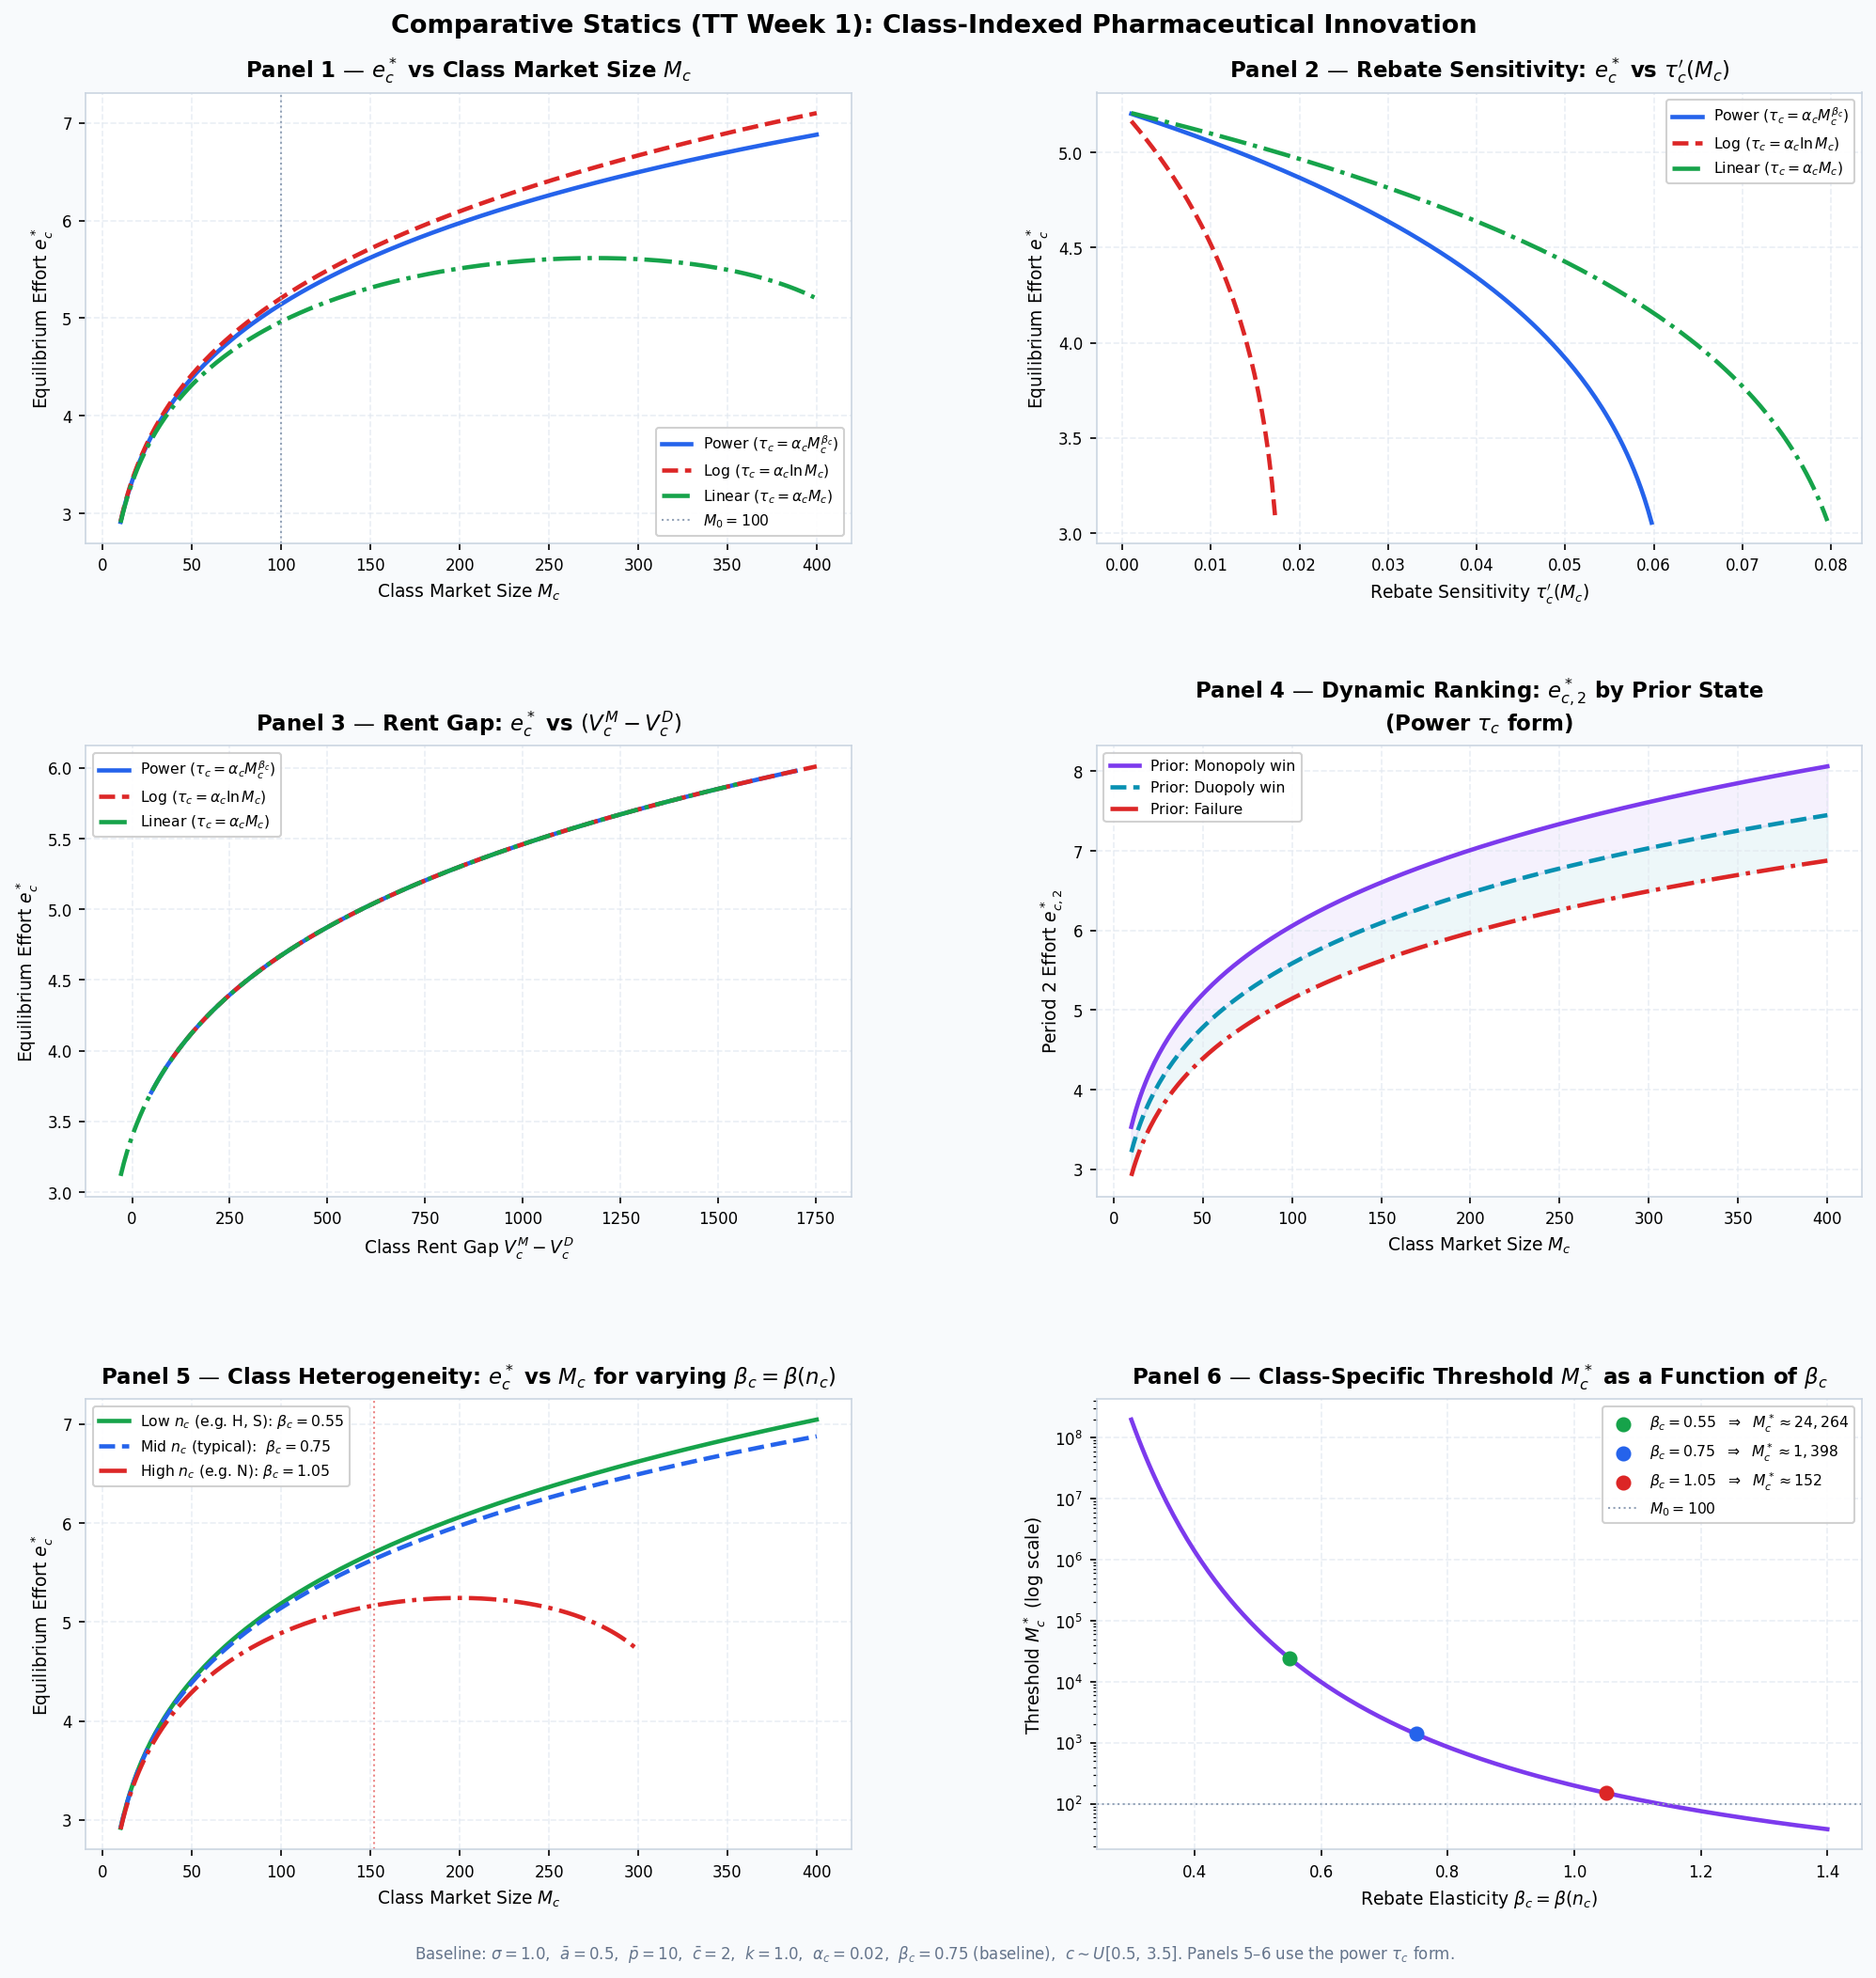
\includegraphics[width=\textwidth]{TT_week1_model.png}
    \caption{Comparative statics of equilibrium effort $e_c^*$. Baseline parameters: \\ $\sigma = 1.0$, $\bar{a} = 0.5$, $\bar{p} = 10$, $\bar{c} = 2$, $k = 1.5$, $\alpha_c = 0.02$, $\beta_c = 0.75$, $c \sim U[0.5, 3.5]$.}
    \label{fig:comp_statics}
\end{figure}

\paragraph{Panel 1: Equilibrium effort and market size.}
The first panel displays $e_c^*$ as a function of market size $M_c$ for each $\tau_c(M_c)$ specification. Under the logarithmic and power forms ($\beta_c = 0.75$), effort rises monotonically with $M_c$ indicating that the volume effect dominates the rebate effect, that is, the additional revenue from serving a larger market dominates, and firms invest more in R\&D as the market expands. The linear form, however, produces a hump-shaped profile. Effort initially increases with $M_c$ but subsequently declines, tracing out precisely the incentive trap mechanism. This shift occurs since the linear rebate schedule $\tau_c = \alpha_c M_c$ implies a constant marginal rebate rate, so the monopsony extraction grows one-for-one with market size. Once $M_c$ is large enough, the term $M_c\tau_c'(M_c) = \alpha_c M_c$ dominates the volume gain $(\bar{p} - \bar{c} - \tau_c)$, so $dV_c^M/dM_c < 0$ and the marginal benefit of effort falls.

In the class-indexed framework, different therapeutic classes correspond to different positions along the horizontal axis and different rebate steepnesses. The empirical results (with class P excluded; see Section \ref{sec:rq3_mapping}) suggest that the majority of classes operate in the upward-sloping region where the volume effect dominates, while a small number of high-volume, therapeutically competitive classes (most notably N) sit near or just past the peak of the hump-shaped profile.

\paragraph{Panel 2: Equilibrium effort and rebate sensitivity.}
The second panel holds $M_c$ fixed at the baseline value $M_0 = 100$ and varies the rebate scale parameter $\alpha_c$, therefore mapping the resulting $\tau_c'(M_c)$ against equilibrium effort $e_c^*$ and isolating the monopsony channel. Across all three $\tau_c$ specifications, equilibrium effort is strictly decreasing in $\tau_c'(M_c)$. Irrespective of functional form, the direction of the effect is unambiguous, and the magnitude is governed by how aggressively $\tau_c$ responds to market size.

The curves diverge substantially in the rate of decline. The logarithmic form exhibits the steepest collapse, while the linear and power forms sustain higher efforts across a wider range of sensitivity values before $V_c^M$ is fully eroded. In the cross-class interpretation, classes with more therapeutic substitutes (higher $n_c$) face steeper effective rebate sensitivity and correspondingly lower equilibrium effort.

\paragraph{Panel 3: Equilibrium effort and the rent gap.}
The third panel varies the price cap $\bar{p}$ to trace equilibrium effort $e_c^*$ as a function of the rent gap $V_c^M - V_c^D$. It shows that innovation is driven by the gap between monopoly and duopoly payoffs, rather than by the level of either payoff alone. Because the first-order condition depends on this rent differential, the relationship between $e_c^*$ and $V_c^M - V_c^D$ is independent of the specific rebate functional form, which is why the curves overlap. Any policy that compresses the monopoly premium --- through a higher rebate wedge, a lower price cap, or stronger competition in procurement --- lowers equilibrium effort.

This panel is particularly important for the class-heterogeneity framework: it establishes that the rent gap $\Delta V_c = V_c^M - V_c^D$ is the sufficient statistic for innovation effort, regardless of the functional form of $\tau_c$. The cross-sectional variation in innovation responses across classes is therefore driven by variation in $\Delta V_c$, not by $M_c$ alone.

\paragraph{Panel 4: Period 2 effort by prior state.}
The fourth panel illustrates the dynamic ranking result under the power specification $\tau_c(M_c)=\alpha_c M_c^{\beta_c}$. For each value of $M_c$, period 2 equilibrium effort is computed under three cost parameters corresponding to the three possible period 1 outcomes: a monopoly win, a duopoly win, and failure. The ranking
\[
e_{c,2}^*(V_c^M) > e_{c,2}^*(V_c^D) > e_{c,2}^*(0)
\]
holds throughout. This is consistent with the model's dynamic mechanism: firms that secure higher rents in period 1 face lower effective R\&D costs in period 2 and therefore invest more in subsequent innovation. The gaps between the three paths widen with market size, showing that the long-run innovation consequences of period 1 procurement outcomes become stronger in larger markets.

In the class-indexed framework, this panel has an additional cross-sectional interpretation. In near-threshold classes such as N, where $V_c^M$ is partially compressed, the three curves are closer together: PDL winners enjoy a smaller cost advantage over non-winners. In volume-dominated classes (the majority), the curves are widely separated, and the winner advantage is large.

Taken together, the four panels provide a consistent picture of the model's predictions. The incentive trap arises once rebate growth with market size is sufficiently strong. Innovation appears to be governed by the rent gap $(V_c^M - V_c^D)$ rather than by any functional form of $\tau_c(M_c)$. The dynamic extension further shows that these effects persist over time, since weaker current rents translate into weaker future innovation incentives. The class-indexed structure determines \textit{which} classes fall into each regime.

\subsection{Theoretical States and Empirical Outcomes}

To bridge the theoretical framework with the empirical analysis, the regression variables are mapped directly to the realised outcomes of the game's two-hurdle structure.

\subsubsection{Mapping to the PDL Counterfactual (RQ2)}

Empirically, the pharmaceutical procurement pipeline is observed through three sequential indicators: passing clinical approval, submitting a pricing bid, and ultimately gaining preferred status. In the context of the model, these variables represent different realised ex-post paths of partial versus full success:

\begin{itemize}
    \item \textbf{Full Market Access:} These are firms that secure the Monopoly state (Stage 3a) or actually win the Duopoly auction (Stage 3b). In this scenario, they clear all hurdles and capture the market $M_c$. They benefit from both channels of state-dependent innovation: they accumulate regulatory know-how while also realising a strictly positive ex-post internal cash flow ($V_c^M$ or $V_c^D$). Consequently, they secure a strictly lower marginal cost of future R\&D effort ($k(V_c^M)$ or $k(V_c^D)$), allowing them to overcome market disincentives.
    
    \item \textbf{Partial Success:} These represent firms that exert sufficient effort to clear the clinical stage ($a_{i,c} \ge \bar{a}$) and enter the price stage (Stage 3b), but ultimately lose to a lower bidder in the bidding game. While clearing the clinical hurdle provides these firms with some accumulated regulatory know-how, the auction uncertainty has converged to failure. They capture zero volume and realise an ex-post payoff of zero ($\pi_{i,c,1} = 0$). Due to receiving no internal cash flows to alleviate capital market frictions, their cost parameter remains strictly higher than that of the PDL winners, falling in some intermediate interval $k \in (k(V_c^D), k(0))$. This relative cost disadvantage causes subsequent innovation to decline once combined with rebate disincentives.
\end{itemize}

The negative coefficients on the partial success stages capture the aggregate disincentive caused by the Medicaid expansion. Following the ACA expansion, states leveraged their expanded market size $M_c$ to extract deeper monopsony rebates $\tau_c(M_c)$, resulting in expected profits collapsing. Firms that reach these intermediate stages expend the cost of effort to clear the hurdles, but realise no cash flows, so their subsequent R\&D efforts decline.

Conversely, the highly positive coefficient on full market access is driven by state-dependent innovation. Firms that actually gain PDL status secure the internal cash flows required to bypass capital market frictions. This influx of capital strictly lowers their future cost of effort parameter ($k$). For these winners, the reduction in the marginal cost of R\&D effort outweighs the aggregate marginal benefit compression, resulting in a net increase in subsequent innovation effort relative to their off-PDL rivals.

\subsubsection{Mapping to the Triple-Difference (RQ3)} \label{sec:rq3_mapping}

The RQ3 specification estimates:
\begin{equation}
    Y_{f,c,t} = \alpha_f + \lambda_c + \delta_t + \sum_{c \in \mathcal{C}} \beta_c \cdot \mathbb{1}\{t \geq 2014\} \cdot \text{MedicaidShare}_c \cdot \mathbb{1}\{\text{ATC} = c\} + \varepsilon_{f,c,t}
\end{equation}

The coefficient $\beta_c$ captures the differential effect of expansion on innovation in class $c$, scaled by that class's Medicaid exposure. Class P (antiparasitic products, insecticides and repellents) is excluded from the analysis: this class exhibited implausibly large coefficients and standard errors (e.g.\ $+62.081$ for patents, $-144.262$ for FDA approvals), driven by extremely thin cell counts, and its inclusion distorted patent estimates across all other classes. Substantively, antiparasitic products are largely over-the-counter and do not pass through the typical PDL procurement channel that the model describes; their exclusion is therefore justified on both statistical and institutional grounds.

The model generates the following mapping between the theoretical regime and the empirical DDD coefficient:

\begin{table}[h]
\centering
\begin{tabular}{llll}
\hline
\textbf{Regime} & \textbf{Condition} & \textbf{Prediction} & \textbf{Empirical sign of $\beta_c$} \\
\hline
Volume-dominated & $M_c^{post} < M_c^*$ & $de_c^*/d\Delta M_c > 0$ & $\beta_c > 0$ \\
Near-threshold   & $M_c^{post} \approx M_c^*$ & $de_c^*/d\Delta M_c \approx 0$ & $\beta_c \approx 0$ \\
Trap-bound       & $M_c^{post} > M_c^*$ & $de_c^*/d\Delta M_c < 0$ & $\beta_c < 0$ \\
\hline
\end{tabular}
\caption{Mapping between the theoretical regime and the empirical DDD coefficient $\beta_c$.}
\label{tab:regime_mapping}
\end{table}

With class P excluded, the patent coefficients (ex-ante exposure) are as follows: B ($+2.269^{***}$), D ($+7.921^{***}$), G ($+4.803^{***}$), H ($+12.926^{***}$), J ($+3.124^{***}$), L ($+15.201^{***}$), R ($+0.298^{***}$), S ($+1.556^{***}$), C ($+0.590^{**}$), M ($+1.660^{**}$), A ($+0.252$, insignificant), and N ($-0.015$, insignificant). The FDA approval coefficients are unchanged from the specification including P.

The empirical classification is:
\begin{itemize}
    \item \textbf{Volume-dominated} (B, C, D, G, H, J, L, M, R, S): These classes exhibit significantly positive $\beta_c$ coefficients, indicating that $M_c^{post} < M_c^*$ and the standard market-size effect dominates. The expansion increased both utilisation and innovation incentives in these therapeutic areas, consistent with the predictions of \cite{garthwaite2021markets}.
    
    \item \textbf{Near-threshold} (A, N): These classes show statistically insignificant coefficients close to zero. The volume and monopsony effects approximately cancel ($M_c^{post} \approx M_c^*$). Notably, N (nervous system) is among the largest Medicaid classes by utilisation volume and has a high degree of therapeutic substitutability - precisely the combination of conditions under which the model predicts the threshold is most likely to be approached.
\end{itemize}

\paragraph{Reconciling the class-level and aggregate results.}
The aggregate RQ1 specification shows a significant decline in patenting among firms in higher-Medicaid-share classes post-expansion, while the class-level RQ3 decomposition reveals that nearly all individual classes experience positive or null effects. This apparent contradiction is explained by the different estimators the two specifications employ.

The RQ1 specification uses firm$\times$class fixed effects and interacts a single class-level MedicaidShare variable with year indicators, imposing a common slope across all therapeutic areas. The RQ3 specification uses separate firm and class fixed effects, and saturates the post$\times$MedicaidShare interaction with ATC class indicators, allowing each class its own slope. These are not nested specifications: they absorb different sources of variation and weight the data differently. In particular, the pooled RQ1 estimator constrains classes with very different innovation responses to share a single coefficient, and the resulting estimate is sensitive to the distribution of Medicaid exposure shares across classes.

The class-indexed model provides the interpretive framework for understanding why pooling produces a negative result. The theoretical prediction is that the incentive trap activates selectively --- only in classes where the combination of large $\Delta M_c$ and high therapeutic substitutability $n_c$ pushes the market toward the threshold $M_c^*$. In most classes, the volume effect dominates and innovation rises with market size, consistent with standard theory. But the pooled specification cannot distinguish between these heterogeneous responses: by constraining them to a single slope, it produces an aggregate coefficient that obscures the class-level pattern.

In the structure of the thesis, the aggregate RQ1 result therefore serves as the motivating puzzle: the negative pooled coefficient contradicts the standard market-size prediction of \cite{garthwaite2021markets} and raises the question of why a larger public market might not translate into greater innovation. The RQ3 decomposition and the theoretical model then provide the answer: the aggregate is misleading because it pools together genuinely positive responses in volume-dominated classes with near-threshold responses in high-weight classes. The thesis contribution is to show that this aggregation conceals economically meaningful heterogeneity driven by the procurement institutions --- specifically, the steepness of the rebate schedule --- attached to each therapeutic area.

\subsubsection{Additional Testable Implications}

The class-indexed model generates several testable implications beyond the sign pattern of $\beta_c$:

\begin{enumerate}
    \item \textbf{Substitutability and threshold proximity.} Classes near the threshold (A, N) should have higher therapeutic substitutability $n_c$ than volume-dominated classes, conditional on Medicaid exposure. This is directly testable using counts of PDL-eligible molecules per class.
    
    \item \textbf{Class-specific rebate elasticities.} The rebate--market size regression ($\tau$ on $\log M$) should yield larger coefficients in near-threshold classes than in volume-dominated classes, since classes approaching the threshold are predicted to have the steepest rebate schedules.
    
    \item \textbf{Winner advantage heterogeneity.} The coefficient on PT\_Pass $\times$ Price\_Pass $\times$ Post (the PDL winner advantage from RQ2) should be largest in volume-dominated classes and smallest in near-threshold classes, consistent with Result \ref{res:dynamic}. In near-threshold classes where $V_c^M$ is partially compressed, even PDL winners accumulate less surplus, weakening the dynamic advantage.
    
    \item \textbf{Aggregate weight decomposition.} A formal decomposition of the aggregate RQ1 coefficient into class-specific contributions (weighting $\beta_c$ by each class's share of the Medicaid market) should confirm that the aggregate decline is disproportionately driven by the near-threshold classes, particularly N.
\end{enumerate}

\subsection{Policy Implications}
The model highlights a central policy trade-off in public pharmaceutical procurement that is now understood to be class-specific. As the Medicaid market size expands, states are able to negotiate deeper supplemental rebates and thereby reduce current expenditure. However, if these rebates compress monopoly rents too aggressively, they also weaken the returns to successful innovation and reduce firms' incentives to invest in R\&D.

The class-level decomposition reveals that this trade-off is empirically relevant only at the margin. In the vast majority of therapeutic classes, the volume effect dominates and the Medicaid expansion has increased innovation incentives alongside access - the standard \cite{garthwaite2021markets} prediction holds. The incentive trap binds selectively, primarily in the highest-volume, most therapeutically competitive classes (notably N, nervous system) where the combination of large $\Delta M_c$ and high $n_c$ pushes $M_c^{post}$ toward the threshold $M_c^*$.

This selectivity has important implications for policy design. A blanket policy response to the aggregate innovation decline - such as uniformly limiting supplemental rebates - would be poorly targeted. In volume-dominated classes (the overwhelming majority), the expansion is working as intended: increasing both access and innovation incentives. Uniform rebate caps in these classes would reduce fiscal savings from competitive procurement without addressing any innovation shortfall.

The relevant policy question is narrower: how to design procurement institutions in near-threshold classes that preserve the fiscal benefits of competitive rebate negotiation while preventing the rebate wedge from growing so steeply that it fully offsets the volume effect. The model points to two distinct policy margins:

The first operates through expected returns: procurement design determines the payoff from successful innovation through the rebate wedge $\tau_c(M_c)$. In near-threshold classes such as N, policies that cap the marginal rebate rate $\tau_c'(M_c)$ or provide preferential treatment for genuinely novel molecules could prevent $M_c^{post}$ from crossing $M_c^*$.

The second operates through the cost of innovation: firms' incentives can also be supported by lowering the effective cost of effort $k$, for example through R\&D subsidies, tax credits, or policies that reduce the cost of clinical development. Targeted subsidies in near-threshold classes could offset the partial rent compression experienced by firms in those areas.

The aggregate decline in patenting, while driven by a small number of classes, nevertheless has substantial welfare implications because the affected classes (particularly nervous system drugs) represent some of the highest-burden disease areas in the Medicaid population. Even a marginal discouragement of innovation in antidepressants, antipsychotics, or analgesics may have outsized public health consequences. Procurement policy should therefore be assessed not only in terms of immediate fiscal savings, but also in terms of its longer-run effects on pharmaceutical innovation incentives in the specific therapeutic areas most relevant to the insured population.

\newpage

\bibliographystyle{apalike}
\bibliography{references}

\end{document}